%% 
%% Copyright 2019-2024 Elsevier Ltd
%% 
%% This file is part of the 'CAS Bundle'.
%% --------------------------------------
%% 
%% It may be distributed under the conditions of the LaTeX Project Public
%% License, either version 1.3c of this license or (at your option) any
%% later version.  The latest version of this license is in
%%    http://www.latex-project.org/lppl.txt
%% and version 1.3c or later is part of all distributions of LaTeX
%% version 1999/12/01 or later.
%% 
%% The list of all files belonging to the 'CAS Bundle' is
%% given in the file `manifest.txt'.
%% 
%% Template article for cas-dc documentclass for 
%% double column output.

\documentclass[a4paper,fleqn]{cas-dc}

% If the frontmatter runs over more than one page
% use the longmktitle option.

%\documentclass[a4paper,fleqn,longmktitle]{cas-dc}

%\usepackage[numbers]{natbib}
%\usepackage[authoryear]{natbib}
\usepackage[numbers]{natbib}


% Additional packages used by the LWCA manuscript
\usepackage{amsmath}
\usepackage{longtable}
\usepackage{booktabs}
\usepackage{multirow}
\usepackage{array}
\usepackage{graphicx}
\usepackage{url}
\usepackage{hyperref}

\newcommand{\maybeincludegraphics}[2][]{%
\IfFileExists{#2}{\includegraphics[#1]{#2}}{%
\fbox{\parbox{0.92\linewidth}{\centering Figure placeholder: \texttt{#2}}}}}


%%%Author macros
\def\tsc#1{\csdef{#1}{\textsc{\lowercase{#1}}\xspace}}
\tsc{WGM}
\tsc{QE}
%%%

% Uncomment and use as if needed
%\newtheorem{theorem}{Theorem}
%\newtheorem{lemma}[theorem]{Lemma}
%\newdefinition{rmk}{Remark}
%\newproof{pf}{Proof}
%\newproof{pot}{Proof of Theorem \ref{thm}}

\begin{document}
\let\WriteBookmarks\relax
\def\floatpagepagefraction{1}
\def\textpagefraction{.001}

% Short title
\shorttitle{Fine-Tuned LWCA for MI Localization}

% Short author
\shortauthors{S. Mandala et al.}

% Main title of the paper
\title [mode = title]{Fine-Tuned Lead-Wise Channel Attention with SE-Recalibrated CNN--LSTM Transfer Learning for Myocardial Infarction Localization in 12-Lead ECGs}

% Title footnote mark
% eg: \tnotemark[1]
%\tnotemark[1]

% Title footnote 1.
% eg: \tnotetext[1]{Title footnote text}
%\tnotetext[1]{}

% First author
%
% Options: Use if required
% eg: \author[1,3]{Author Name}[type=editor,
%       style=chinese,
%       auid=000,
%       bioid=1,
%       prefix=Sir,
%       orcid=0000-0000-0000-0000,
%       facebook=<facebook id>,
%       twitter=<twitter id>,
%       linkedin=<linkedin id>,
%       gplus=<gplus id>]

\author[1,2]{Satria Mandala}

% Corresponding author indication
\cormark[1]

% Footnote of the first author
%\fnmark[1]

% Email id of the first author
\ead{satriamandala@telkomuniversity.ac.id}

% URL of the first author

% Credit authorship
% eg: \credit{Conceptualization of this study, Methodology, Software}
\credit{Methodology, Supervision, Writing--review and editing}

% Address/affiliation
\affiliation[1]{organization={Telkom University},
            addressline={},
            city={Bandung},
%          citysep={}, % Uncomment if no comma needed between city and postcode
            postcode={40257},
            state={West Java},
            country={Indonesia}}

\affiliation[2]{organization={Human Centric (HUMIC) Engineering, Telkom University},
            addressline={},
            city={Bandung},
%          citysep={}, % Uncomment if no comma needed between city and postcode
            postcode={40257},
            state={West Java},
            country={Indonesia}}



% Address/affiliation
\affiliation[3]{organization={Center for Intelligent Cloud Computing, COE for Advanced Cloud, Multimedia University},
            addressline={},
            city={Melaka},
%          citysep={}, % Uncomment if no comma needed between city and postcode
            postcode={75450},
            state={},
            country={Malaysia}}

\affiliation[4]{organization={Centre for Advanced Analytics, COE for Artificial Intelligence, Multimedia University},
            addressline={},
            city={Melaka},
%          citysep={}, % Uncomment if no comma needed between city and postcode
            postcode={75450},
            state={},
            country={Malaysia}}

\affiliation[5]{organization={Faculty of Information Science and Technology, Multimedia University},
            addressline={},
            city={Melaka},
%          citysep={}, % Uncomment if no comma needed between city and postcode
            postcode={75450},
            state={},
            country={Malaysia}}

\affiliation[6]{organization={Faculty of Engineering and Technology, Multimedia University},
            addressline={},
            city={Melaka},
%          citysep={}, % Uncomment if no comma needed between city and postcode
            postcode={75450},
            state={},
            country={Malaysia}}

\author[1]{Nugroho Rahmanto}
\credit{Software, Validation, Formal analysis, Investigation, Writing--original draft}

\author[3,5]{Sharifah Noor Masidayu Sayed Ismail}
\credit{Methodology, Validation, Writing--review and editing}

\author[4,6]{Nor Azlina Ab Aziz}
\credit{Validation, Supervision, Writing--review and editing}

\author[3,5]{Siti Fatimah Abdul Razak}
\credit{Validation, Writing--review and editing}

\author[1]{Jondri}
\credit{Supervision, Writing--review and editing}

\author[1]{Eko Darwiyanto}
\credit{Supervision, Writing--review and editing}

% Corresponding author text
\cortext[1]{Corresponding author.}

% Footnote text
%\fntext[1]{}

% For a title note without a number/mark
%\nonumnote{}

% Here goes the abstract
\begin{abstract}
Accurate myocardial infarction (MI) localization from 12-lead electrocardiograms remains challenging because infarct evidence is lead-dependent, temporally localized, and affected by severe minority-class scarcity. This study proposes a fine-tuned Lead-Wise Channel Attention (LWCA) framework integrated with a CNN--LSTM encoder, multi-stage squeeze-and-excitation (SE) recalibration, and temporal attention pooling. LWCA estimates sample-specific lead importance before morphological feature extraction, while SE blocks recalibrate latent convolutional channels so that lead-modulated representations remain selective across deeper feature levels. The model is pretrained on PTB-XL and fine-tuned on PTB Diagnostic ECG for four-class localization: normal rhythm (NORM), anterior MI (AMI), inferior MI (IMI), and lateral MI (LMI). We compare scratch training, frozen-backbone transfer, partial fine-tuning, full fine-tuning, local pretrained CNN1D/CNN--LSTM/GRU/LSTM baselines, external ECG foundation models (HuBERT-ECG and ECG-FM), and GAN-assisted LMI augmentation. Without GAN augmentation, LWCA partial fine-tuning achieves an average test macro-F1 of 0.7889 across five folds and 0.8954 in the best fold using 0.95M total parameters and 0.45M trainable parameters. ECG-FM obtains a higher no-GAN average macro-F1 of 0.8334 but requires 90.89M trainable parameters. With GAN-assisted leave-one-LMI augmentation, LWCA improves to 0.8574 macro-F1 with partial fine-tuning and 0.8653 with full fine-tuning, reaching 0.9688 in the best fold. These results indicate that lead-wise attention, SE recalibration, and fine-tuning strategy jointly improve imbalanced MI localization. \textbf{GitHub Repository:} \href{https://github.com/NugrohoRahmanto/myocardial-infarction-classification}{https://github.com/NugrohoRahmanto/myocardial-infarction-classification}
\end{abstract}

% Use if graphical abstract is present
%\begin{graphicalabstract}
%\includegraphics{}
%\end{graphicalabstract}

% Research highlights
\begin{highlights}
\item A Lead-Wise Channel Attention module is proposed for compact 12-lead MI localization.
\item SE blocks recalibrate latent CNN channels after lead-aware input modulation.
\item No-GAN, GAN-assisted, local baseline, HuBERT-ECG, and ECG-FM comparisons are reported using fold-level macro-F1.
\item GAN-assisted full fine-tuning reaches 0.8653 average macro-F1 and 0.9688 best-fold macro-F1.
\end{highlights}


% Keywords
% Each keyword is seperated by \sep
\begin{keywords}
Myocardial infarction \sep 12-lead ECG \sep Lead-wise channel attention \sep Squeeze-and-excitation \sep Fine-tuning \sep ECG foundation model \sep GAN augmentation
\end{keywords}

\maketitle

% Main text
% \section{}\label{}

% Numbered list
% Use the style of numbering in square brackets.
% If nothing is used, default style will be taken.
%\begin{enumerate}[a)]
%\item
%\item
%\item
%\end{enumerate}

% Unnumbered list
%\begin{itemize}
%\item
%\item
%\item
%\end{itemize}

% Description list
%\begin{description}
%\item[]
%\item[]
%\item[]
%\end{description}

% Figure
%\begin{figure}%[]
%  \centering
%    \includegraphics{}
%    \caption{}\label{fig1}
%\end{figure}

% Table
%\begin{table}%[]
%\caption{}\label{tbl1}
%\begin{tabular*}{\tblwidth}{@{}LL@{}}
%\toprule
%  &  \\ % Table header row
%\midrule
% & \\
% & \\
% & \\
% & \\
%\bottomrule
%\end{tabular*}
%\end{table}

%%
%% Start line numbering here if you want
%%
% \linenumbers

%% main text
% \section{}
% \label{}

\section{Introduction}
Myocardial infarction (MI) remains a major cause of acute cardiovascular morbidity and mortality, and the 12-lead electrocardiogram (ECG) continues to be the most accessible first-line examination for rapid clinical assessment. Beyond detecting MI, localizing the infarct territory is clinically important because anterior MI (AMI), inferior MI (IMI), and lateral MI (LMI) are associated with different lead involvement patterns and may imply different downstream clinical considerations. Automated MI localization is therefore not merely a multi-class classification problem; it is a lead-sensitive interpretation task in which diagnostic evidence may be sparse, subtle, and distributed unevenly across the standard 12-lead configuration.

Deep learning has improved ECG analysis by enabling end-to-end representation learning from raw signals. Large resources such as PTB-XL have supported supervised pretraining and benchmarking at scale \cite{Wagner2020SciData_PTBXL,StrodthoffWagnerSchaeffterSamek2021JBHI_PTBXL_Benchmarks}, while smaller clinical datasets such as the PTB Diagnostic ECG Database remain important for target-domain evaluation \cite{Bousseljot1995PTB,Goldberger2000PhysioBank}. However, cross-dataset transfer remains challenging because acquisition conditions, label definitions, class priors, and patient distributions differ across cohorts. In MI localization, these difficulties are amplified by severe class imbalance. LMI is particularly scarce in many public subsets, making macro-F1 more informative than accuracy because accuracy can remain high even when minority infarct territories are missed.

Recent ECG models have explored CNNs, recurrent networks, attention mechanisms, and foundation-model pretraining. CNNs provide local morphology extraction, LSTMs and GRUs model temporal dependencies, and attention mechanisms can emphasize relevant signal components \cite{FengPiLiuSun2019ApplSci_MI_CNN_RNN,Hasbullah2023BioMedInformatics_MI_Hybrid_CNN_RNN,Cao2022FrontPhysiol_MSResNet_Attn_MI}. In parallel, large external ECG foundation models such as HuBERT-ECG and ECG-FM have introduced self-supervised pretraining at scale \cite{HuBERTECG2024,McKeen2024ECGFM}. These models are powerful, but their downstream effectiveness depends on the compatibility between the pretraining protocol, the fine-tuning strategy, and the target clinical label space. A central question for MI localization is therefore whether a lead-aware CNN--LSTM architecture can be fine-tuned effectively against imported foundation-model representations under a controlled evaluation protocol.

This study addresses that question by reformulating the previously used channel-attention pipeline into a more explicit Lead-Wise Channel Attention (LWCA) framework. LWCA is designed to learn sample-specific lead importance before convolutional morphology extraction. The term ``lead-wise'' is used because the attention weights are assigned to the 12 physiological ECG leads, while ``channel attention'' reflects their role as input channels in the neural network. This distinction is important: LWCA acts on the raw lead dimension, whereas squeeze-and-excitation (SE) blocks act later on learned convolutional feature channels. SE is therefore not used merely as an additional attention layer; it is used to preserve and refine lead-aware information after LWCA has modulated the input, allowing the network to recalibrate latent representations at multiple abstraction levels \cite{Sun2024Sensors_CNNLSTMSE,QuFu2025JSMU_ResLSTM_TemporalSE}.

The contributions of this paper are summarized as follows:
\begin{itemize}
  \item A compact LWCA module is introduced to estimate per-lead relevance from statistical lead descriptors and to adaptively reweight raw 12-lead ECG signals before feature extraction.
  \item SE blocks are repositioned as multi-stage latent channel recalibration units that operate after LWCA, clarifying their role in refining lead-modulated convolutional representations rather than replacing lead attention.
  \item The proposed LWCA--CNN--LSTM--SE architecture is evaluated under PTB-XL to PTB Diagnostic fine-tuning with scratch, frozen-backbone, partial fine-tuning, and full fine-tuning settings.
  \item A comprehensive comparison is reported against local pretrained CNN1D, CNN--LSTM, GRU, and LSTM baselines, and against large external pretrained HuBERT-ECG and ECG-FM models.
  \item The analysis reports average macro-F1 across folds, fold-level details, best-fold behavior, parameter counts, and the effect of GAN-assisted LMI augmentation.
\end{itemize}

\section{Related Work and Research Gap}
\subsection{Deep Learning for ECG and MI Analysis}
ECG interpretation has progressively shifted from handcrafted feature pipelines toward representation learning directly from raw or minimally processed signals. Large-scale benchmarking studies on PTB-XL show that deep architectures can learn clinically meaningful ECG representations when diagnostic labels and evaluation protocols are standardized \cite{Wagner2020SciData_PTBXL,StrodthoffWagnerSchaeffterSamek2021JBHI_PTBXL_Benchmarks}. PTB-XL has also encouraged few-shot and low-resource ECG research, where limited labeled examples create conditions similar to target-domain clinical adaptation \cite{PalczynskiSmigielLedzinskiBujnowski2022Sensors_FewShot_PTBXL}. Earlier PTB-XL classification studies further demonstrate that model performance depends strongly on label granularity and class imbalance \cite{SmigielPalczynskiLedzinski2021Entropy_DL_PTBXL}.

MI-focused ECG studies have investigated both binary detection and localization-oriented formulations. Deep learning has been used for emergency-department MI prediction \cite{Gustafsson2022SciRep_MI_ED}, heartbeat-level classification involving MI and arrhythmia categories \cite{Pham2023Sensors_Heartbeat_ArrMI}, and multi-class MI classification using convolutional and recurrent components \cite{FengPiLiuSun2019ApplSci_MI_CNN_RNN,LuiChow2019IMU_MI_CNN_RNN_Portable,Hasbullah2023BioMedInformatics_MI_Hybrid_CNN_RNN}. These studies motivate hybrid architectures because MI-related ECG evidence may involve both local waveform morphology and temporal evolution over a recording window. However, many existing pipelines treat the 12 leads primarily as homogeneous input channels, whereas clinical MI localization depends on lead-territory relationships. The present work addresses this gap by making lead relevance an explicit learnable component through LWCA.

Beyond MI, broader cardiovascular disease diagnosis has benefited from hybrid deep networks and attention modules. CNN--CBAM--GRU models have been proposed for general cardiovascular disease diagnosis \cite{Gong2025PLOSone_CNN_CBAM_GRU_CVD}, and ensemble-based ECG approaches have been shown to improve arrhythmia detection robustness across multi-lead recordings \cite{MandalaRizalAdiwijayaNurmainiAminiSudarismanHauAbdullah2024PLOSone_Arrhythmia_Ensemble}. These works support the view that multi-lead ECG problems require not only stronger feature extractors but also mechanisms for selective evidence aggregation. The present study follows this direction but focuses specifically on MI localization under severe LMI scarcity.

ECG modeling has also been studied in adjacent cardiovascular screening and deployment contexts. Machine learning has been evaluated for early coronary artery disease prediction \cite{ChenHengjinda2021JAICN_CAD_ML}, wearable systems have been proposed for real-time heart-attack detection and warning \cite{Chowdhury2019Sensors_HeartAttack_Wearable}, and LSTM-based ECG models have been used for personal authentication and continuous wearable monitoring \cite{KimPyun2020Sensors_ECG_Auth_LSTM,SaadatnejadOveisiHashemi2020JBHI_LSTM_Wearable}. These studies reinforce the need for ECG models that are not only accurate but also compact, stable, and suitable for constrained clinical or edge-oriented use cases.

\subsection{Attention, Channel Recalibration, and Temporal Selectivity}
Attention mechanisms have been widely adopted because they provide a learnable strategy for emphasizing discriminative components of high-dimensional signals. In MI detection and localization, multi-scale ResNet with attention has been used to capture infarct-related morphology across temporal resolutions \cite{Cao2022FrontPhysiol_MSResNet_Attn_MI}, while attention-enhanced multi-scale feature optimization has been explored for silent MI and atrial fibrillation detection \cite{Cheng2024AIMLR_Attn_MultiScale_SilentMI_AF}. Multi-domain feature fusion has also been proposed to improve MI detection and localization by integrating complementary representations \cite{Chen2025Biosensors_MDF_Fusion_MI}. These studies indicate that MI evidence is rarely captured optimally by a single uniform feature stream.

Squeeze-and-excitation mechanisms have become important in ECG classification because they allow channel-wise recalibration of learned feature maps. CNN--LSTM--SE models have been used for arrhythmia classification \cite{Sun2024Sensors_CNNLSTMSE}, and ResLSTM-TemporalSE has demonstrated the value of coupling recurrent modeling with SE-style recalibration for multi-lead ECG classification \cite{QuFu2025JSMU_ResLSTM_TemporalSE}. Channel-temporal attention has also been explored in other sequential signal domains, showing that combining channel selectivity with temporal saliency can strengthen discriminative representation learning \cite{LimKim2025ApplSci_SpikeCAN}. In the proposed framework, SE is retained not as a generic attention add-on but as a latent channel recalibration mechanism after explicit physiological lead weighting. This separation is the core distinction of LWCA: lead-level attention and feature-channel recalibration are treated as complementary, not interchangeable.

\subsection{Transfer Learning, Fine-Tuning, and Limited-Label ECG Settings}
Transfer learning is well motivated for ECG because labeled clinical datasets are often smaller than the model capacity required for robust feature extraction. ECG transfer learning has been shown to improve classification performance when source and target domains share relevant morphology \cite{WeimannConrad2021SciRep_TL_ECG,JangKimYoon2021HIR_TL_ECG}. Distant transfer learning across multiple datasets further suggests that representation reuse can improve generalization when domain differences are carefully managed \cite{ChuiGuptaZhaoMalibariAryaAlhalabiRuiz2022Bioengineering_DistantTL_ECG}. Transfer learning has also been applied to rare ECG-related conditions, illustrating its relevance when target labels are scarce \cite{LopesBleijendaalRamosVerstraelenAminWildePintoDeMolMarquering2021CBM_TL_PLN}. Recent evaluations continue to question when ECG transfer learning is effective, emphasizing that source-target alignment and the selected fine-tuning depth remain critical \cite{NguyenDo2025PLOSone_TL_ECG_Effective}.

The broader machine learning literature reinforces the importance of reusable representations in low-resource target tasks. Unified transfer learning frameworks in natural language processing show that pretraining can be highly effective when downstream adaptation is carefully designed \cite{RaffelShazeerRobertsLeeNarangMatenaZhouLiLiu2020JMLR_T5}. Similar principles have been adopted in physiological signal research, including MI identification from phonocardiogram signals using segmented features and transfer learning \cite{MandalaAminiAdiwijayaSyaifullahPramudyoNurmainiAbdullah2023IEEEAccess_PCG_MI_TL}. Although such works differ in modality, they support the general hypothesis that source-domain representation learning can stabilize target-domain classifiers when fine-tuning is matched to the downstream task. This paper tests that hypothesis specifically for 12-lead MI localization, while also comparing LWCA fine-tuning against large imported ECG foundation models.

\subsection{Signal Processing Context and Broader Feature-Learning Evidence}
Reliable physiological classification depends not only on model architecture but also on signal representation, denoising, and feature stability. Prior work on ECG denoising with Daubechies wavelets \cite{MandalaFuadahArzakiPambudi2017ICoICT_ECG_Denoising,MandalaTresnasariLestari2022ICICyTA_ECG_Daubechies} and analysis of wavelet basis functions for ECG-based artificial intelligence \cite{MandalaWibowoAdiwijayaSuyantoZahidRizal2023ApplSci_DWBF_AF} shows that preprocessing choices can materially affect downstream model behavior. Related work on malignant ventricular arrhythmia prediction and review of ECG parameters further highlights the clinical importance of robust ECG feature selection \cite{MandalaCaiDiSunarAdiwijaya2020PLOSone_MVA_DecisionTree,MandalaCaiDi2017JMBE_MVA_Review}. Adjacent physiological-signal studies using PPG and PCG demonstrate that denoising, segmentation, and handcrafted feature design remain valuable references for deep-learning pipelines \cite{ParsaoranMandalaPramudyo2022ICoDSA_PPG_Denoising,IhsanMandalaPramudyo2022ICoDSA_PPG_CHD,IqtidarQamarAzizKhan2021CBM_PCG_CAD}.

Feature learning principles also extend beyond cardiac signals. Hybrid feature extraction for facial expression recognition \cite{KommineniMandalaSunarChakravarthy2021JSC_FER_Hybrid}, image preprocessing for content-based retrieval \cite{KommineniMandala2014ICACCI_CBirPreprocess}, CNN-based smart home recognition \cite{MandalaRamadhanIrsan2023COMNETSAT_SmartHome_CNN}, LSTM transfer learning for building energy demand \cite{Kim2023Sustainability_LSTMTL_Energy}, and LSTM-based radio-frequency signal identification \cite{Wang2020CSSP_LSTM_TL_RF} all indicate that selective representation learning and domain adaptation are recurring issues across signal-processing applications. These studies provide broader methodological context for the present work: LWCA is a task-specific instance of selective representation learning, designed for the anatomical and diagnostic structure of 12-lead ECG.

\subsection{Research Gap}
The literature suggests four unresolved gaps. First, MI localization remains more difficult than general MI detection because lead-territory relationships must be modeled explicitly. Second, many attention-based ECG models emphasize latent feature maps but do not distinguish physiological lead weighting from learned feature-channel recalibration. Third, imported foundation models may provide strong representations, but their effectiveness depends on downstream fine-tuning and task alignment. Fourth, rare-class behavior, especially LMI, requires reporting beyond accuracy and should be evaluated using fold-level macro-F1 and augmentation-aware protocols. The proposed LWCA framework is designed around these gaps by combining explicit lead attention, SE-based latent recalibration, PTB-XL pretraining, controlled fine-tuning strategies, and no-GAN/GAN comparative evaluation.

\section{Data Resources and Experimental Protocol}
\subsection{Source and Target ECG Datasets}
The source domain is PTB-XL, a large clinical 12-lead ECG dataset with standardized diagnostic annotations and sufficient scale for representation learning \cite{Wagner2020SciData_PTBXL}. The target domain is the PTB Diagnostic ECG Database, a smaller clinical ECG collection that is suitable for evaluating target-domain adaptation under sample scarcity and class imbalance \cite{Bousseljot1995PTB}. Both datasets are harmonized into four MI localization categories: NORM, AMI, IMI, and LMI.

All ECGs are represented as raw 12-lead time-series segments with a sampling frequency of 100 Hz and a fixed duration of 10 s, resulting in 1000 samples per lead. This unified representation ensures that the source and target models share an identical input dimensionality. The use of raw 10 s windows is intentionally retained to avoid dependence on beat segmentation, which can introduce additional failure modes when QRS detection is affected by noise, baseline drift, or abnormal morphology. The input tensor therefore preserves the complete temporal context available to the model.

The reported target-domain experiments use a held-out test set of 42 ECG recordings with class support NORM=16, AMI=9, IMI=16, and LMI=1. The remaining target-domain data are used for fold-wise model development. Because the held-out LMI support contains one sample, all LMI-specific conclusions are interpreted cautiously; macro-F1 is emphasized to reduce majority-class dominance. This setting is deliberately stringent: it reflects the practical situation in which a model may have to adapt to a small clinical cohort where one infarct territory is severely under-represented. Fig.~\ref{fig:data_distribution_ring} summarizes the class distribution used in the data-understanding stage for PTB Diagnostic and PTB-XL.

\begin{figure}
\centering
\maybeincludegraphics[width=0.86\columnwidth]{figs/data_distribution_ring_chart.png}
\caption{Ring-chart visualization of class distribution in the prepared PTB Diagnostic and PTB-XL datasets. The chart highlights the minority status of LMI relative to the remaining classes and motivates the use of macro-F1 and GAN-assisted LMI evaluation.}
\label{fig:data_distribution_ring}
\end{figure}

\subsection{Label Harmonization and Input Standardization}
The label harmonization procedure maps dataset-specific annotations into the shared four-class target space. NORM represents ECGs without MI evidence, whereas AMI, IMI, and LMI correspond to anterior, inferior, and lateral infarct territories. This mapping is necessary because source and target datasets differ in annotation granularity and class availability. Labels outside the aligned MI localization formulation are excluded to prevent inconsistent supervision during transfer learning.

Before model training, each ECG record is arranged in a fixed lead order corresponding to the standard 12-lead configuration. Records are checked to ensure that the final signal shape is $1000\times12$; transposed files are converted when necessary, and files with incompatible shapes are excluded. In the fold-specific training pipeline, normalization is estimated from the training split only and then applied to validation and test data. This prevents test leakage and ensures that each fold simulates realistic target-domain deployment, where normalization parameters must be learned from available training data.

\subsection{Butterworth Bandpass Inspection}
Butterworth bandpass filtering was used in the data-understanding notebook to inspect the effect of suppressing non-diagnostic frequency components while preserving ECG morphology. A fourth-order Butterworth bandpass with passband 0.5--40 Hz was applied using zero-phase forward--backward filtering. The lower cutoff attenuates baseline wander and slow drift, while the upper cutoff suppresses high-frequency noise that may arise from muscle activity, electrode contact, or acquisition artifacts. The maximally flat Butterworth response is useful for ECG because it avoids passband ripples that can distort morphology-sensitive segments such as QRS complexes, ST-segments, and T-waves. Fig.~\ref{fig:butterworth_raw} shows an example raw Lead II signal and its filtered version, and Fig.~\ref{fig:butterworth_response} shows the corresponding passband behavior.

\begin{figure*}
\centering
\maybeincludegraphics[width=0.88\textwidth]{figs/ecg_raw_vs_butterworth_lead_ii.png}
\caption{Example Lead II ECG visualization before and after fourth-order Butterworth bandpass filtering with a 0.5--40 Hz passband. The filtered signal suppresses slow baseline drift and high-frequency noise while preserving the dominant ECG waveform morphology.}
\label{fig:butterworth_raw}
\end{figure*}

\begin{figure}
\centering
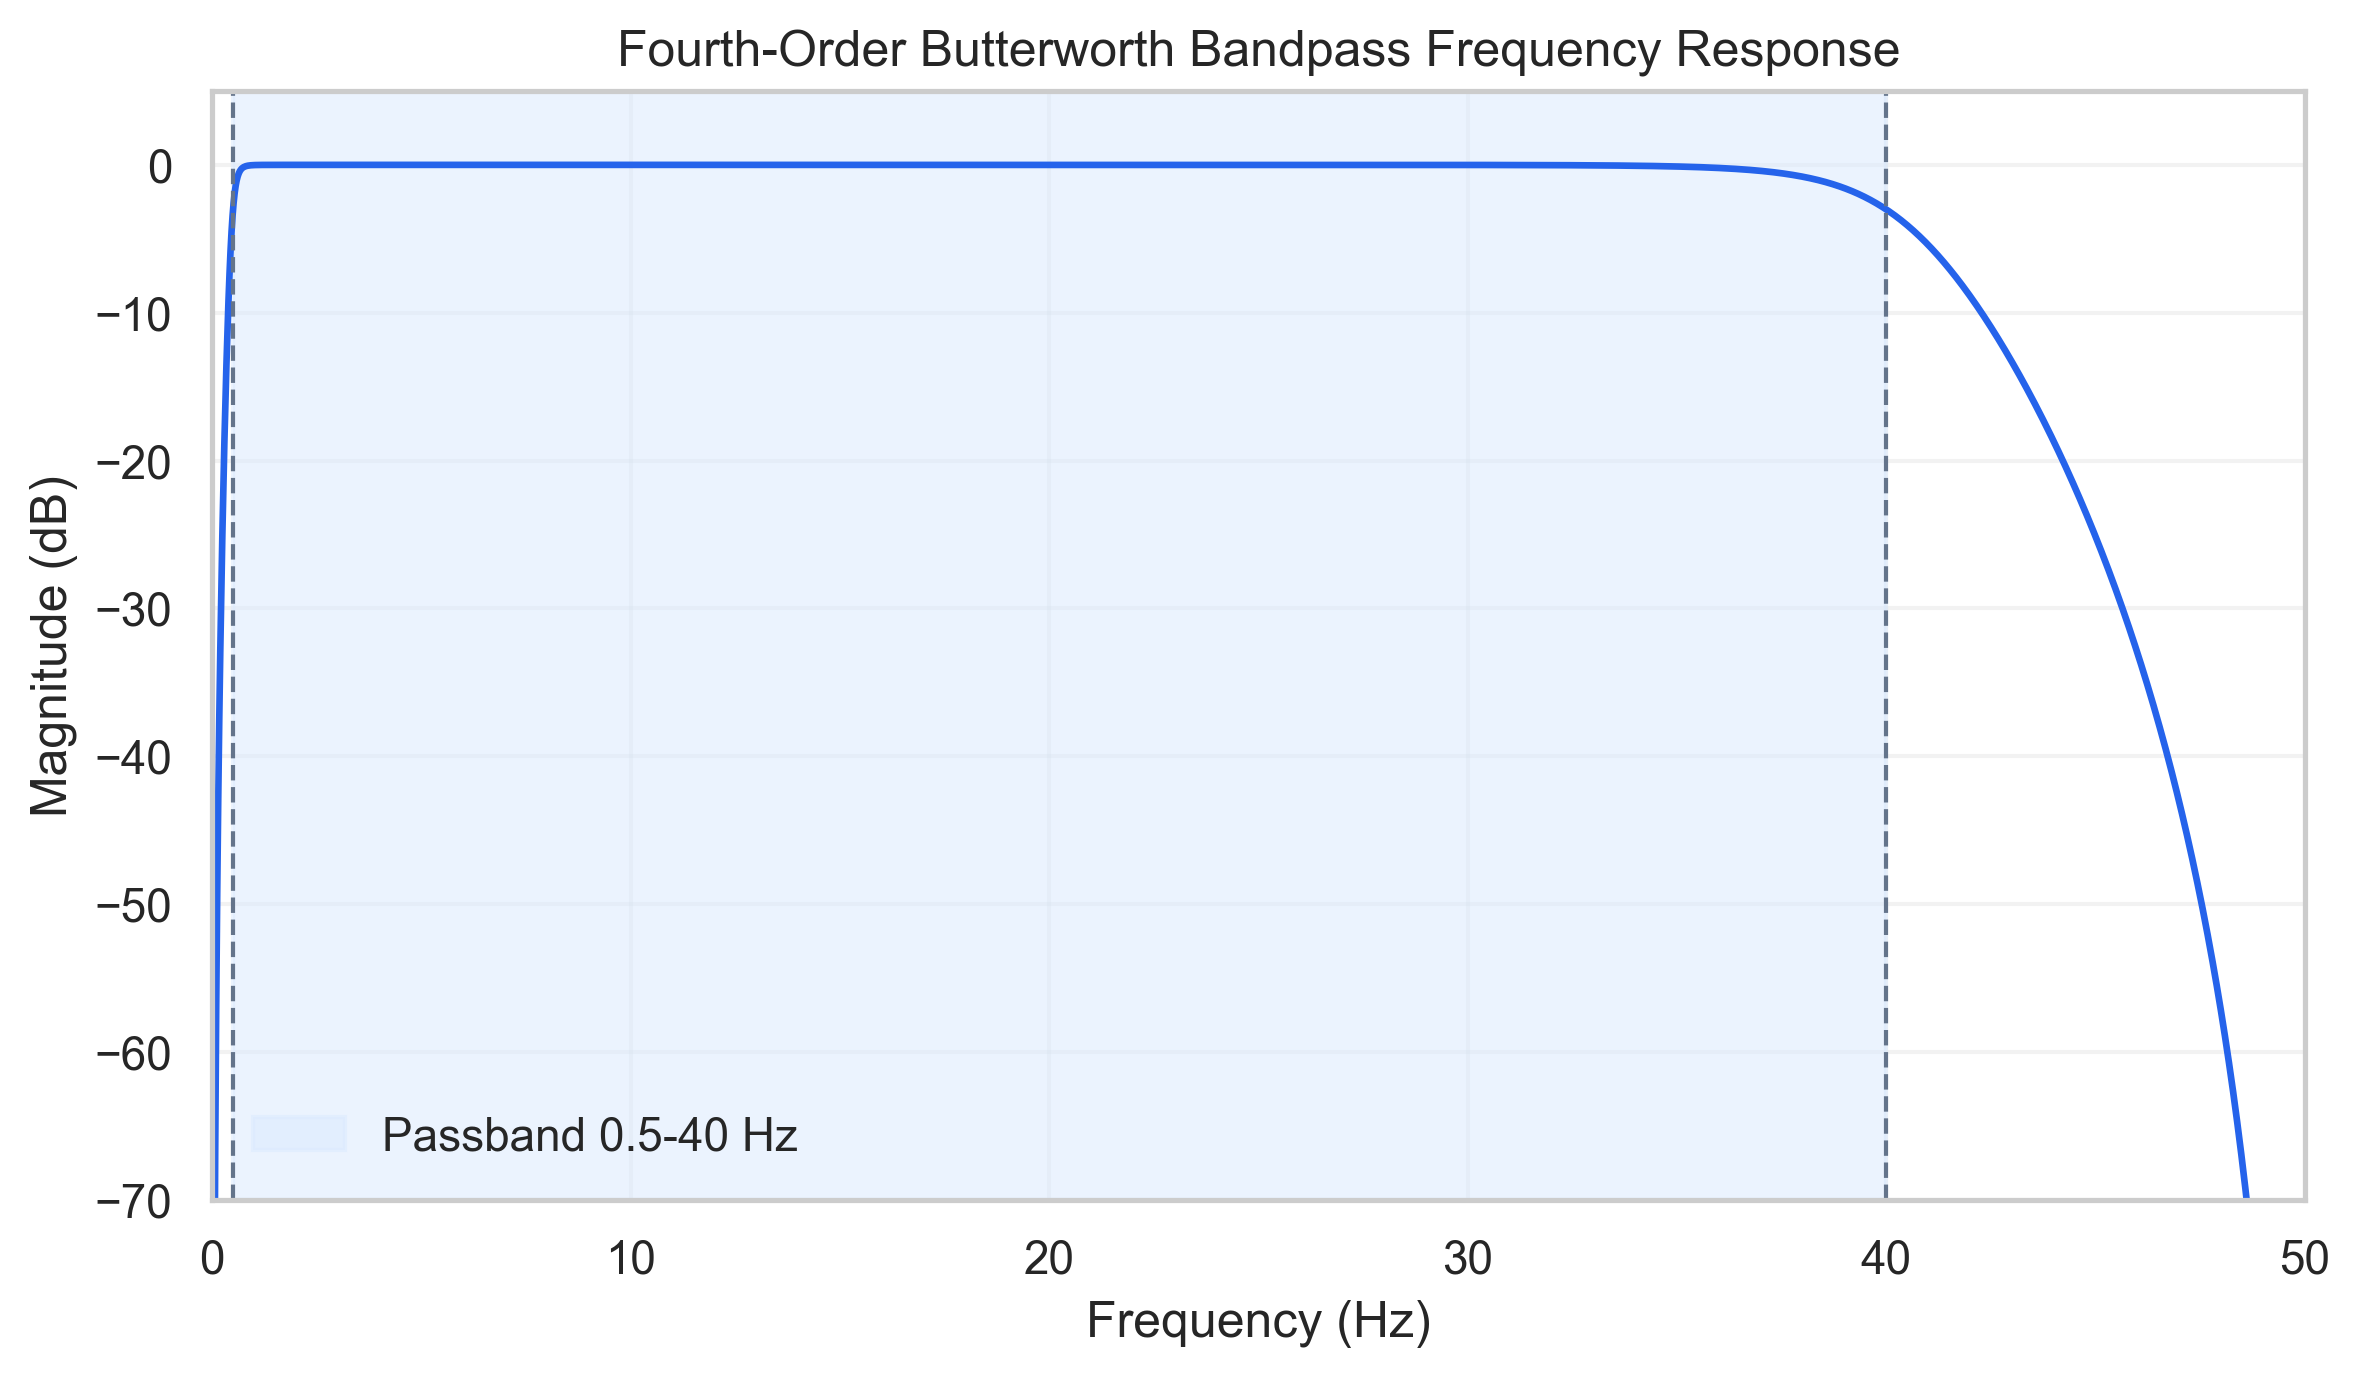
\includegraphics[width=\columnwidth]{figs/butterworth_bandpass_response.png}
\caption{Frequency response of the fourth-order Butterworth bandpass filter used for signal inspection. The 0.5--40 Hz passband retains the main clinical ECG morphology band while attenuating lower-frequency drift and higher-frequency noise.}
\label{fig:butterworth_response}
\end{figure}




\subsection{No-GAN and GAN-Assisted Protocols}
Two experimental regimes are reported. The first regime is the no-GAN setting, where all models are trained or fine-tuned using the available target-domain training folds without synthetic minority augmentation. This regime is used for the main comparison against local pretrained baselines and imported foundation models.

The second regime is a GAN-assisted leave-one-LMI protocol. In this setting, LMI augmentation is used to address the extremely limited LMI availability while preserving an unseen LMI case for evaluation. The protocol evaluates three LMI-centered folds and compares scratch training, frozen-backbone transfer, partial fine-tuning, and full fine-tuning for the LWCA architecture. The purpose is not to claim definitive LMI generalization from a single held-out LMI case, but to quantify whether targeted synthetic augmentation improves fold stability and macro-F1 under a controlled minority-class stress test.

Table~\ref{tab:training_config} summarizes the main training configuration for the no-GAN and GAN-assisted regimes. The same four-class target formulation, validation-based checkpoint selection, and macro-F1-oriented evaluation are retained in both regimes. The key distinction is that the GAN-assisted protocol increases minority-class exposure through LMI synthesis while using a leave-one-LMI evaluation design.

\begin{table*}[!t]
\centering
\caption{Training configuration for no-GAN and GAN-assisted experiments.}
\label{tab:training_config}
\begin{tabular*}{\textwidth}{@{\extracolsep{\fill}}l l l@{}}
\toprule
\textbf{Configuration item} & \textbf{No-GAN protocol} & \textbf{GAN-assisted protocol} \\
\midrule
Target classes & NORM, AMI, IMI, LMI & NORM, AMI, IMI, LMI \\
Input representation & 12 leads, 1000 samples, 10 s & 12 leads, 1000 samples, 10 s \\
Source initialization & PTB-XL pretraining for transfer variants & PTB-XL pretraining for transfer variants \\
Target-domain data & PTB Diagnostic ECG & PTB Diagnostic ECG with synthetic LMI augmentation \\
Fold design & Five validation folds with fixed held-out test set & Three leave-one-LMI folds \\
Adaptation modes & Scratch, frozen, partial, full fine-tuning & Scratch, frozen, partial, full fine-tuning \\
Selection metric & Validation macro-F1 & Validation macro-F1 \\
Primary test metric & Test macro-F1 & Test macro-F1 \\
\bottomrule
\end{tabular*}
\end{table*}

\subsection{Comparison Scope}
The comparison is organized into three levels. The first level evaluates LWCA fine-tuning strategies: scratch training, frozen-backbone transfer, partial fine-tuning, and full fine-tuning. The second level compares LWCA against compact local baselines pretrained or fine-tuned under the same target-domain protocol, including CNN1D, CNN--LSTM, GRU, and LSTM. The third level compares against imported ECG foundation models, namely HuBERT-ECG and ECG-FM. This structure separates three questions: whether LWCA benefits from PTB-XL initialization, which fine-tuning depth is most effective for PTB Diagnostic localization, and how a lead-aware fine-tuned model compares with large pretrained foundation models under the same evaluation metric.

All results are reported at fold level and as mean $\pm$ standard deviation across folds. The best fold is reported separately because it identifies the checkpoint that achieves the strongest target-domain behavior after validation-based selection. The primary comparison is based on test macro-F1 rather than accuracy because the target-domain class distribution is imbalanced and because missing a rare class can have limited effect on accuracy but large clinical relevance.

\section{Methodology}
\subsection{Overall Architecture}
The proposed model receives a raw ECG segment $\mathbf{X}\in\mathbb{R}^{T\times C}$, where $T=1000$ and $C=12$. The architecture consists of four functional components: LWCA for raw-lead weighting, a CNN encoder for morphology extraction, SE blocks for latent feature-channel recalibration, and stacked LSTMs followed by temporal attention pooling for sequence aggregation. Fig.~\ref{fig:lwca_framework} illustrates the full pipeline, and Fig.~\ref{fig:lwca_architecture} summarizes the model components.

The architecture follows a clinically motivated signal-processing order. First, the model estimates which leads are most relevant for the current ECG instance. This is done before convolution because lead importance is a property of the observed 12-lead signal and should influence subsequent morphology extraction. Second, a CNN encoder extracts local waveform patterns such as QRS morphology, ST-segment deviations, and T-wave changes. Third, SE blocks recalibrate the learned feature maps at multiple depths, allowing the network to suppress weak or noisy latent channels and amplify channels that preserve diagnostic evidence. Fourth, LSTM layers integrate the encoded temporal sequence, and temporal attention pooling selects the most informative time regions for classification. The final classifier maps the pooled representation to the four MI localization classes.

\begin{figure}
\centering
\maybeincludegraphics[width=\linewidth]{figs/lwca_framework.png}
\caption{Proposed transfer-learning framework for MI localization. PTB-XL is used for source-domain pretraining, and PTB Diagnostic ECG is used for target-domain adaptation. The reported comparison includes no-GAN training, GAN-assisted LMI augmentation, local pretrained baselines, and imported ECG foundation models.}
\label{fig:lwca_framework}
\end{figure}

\begin{figure}
\centering
\maybeincludegraphics[width=\linewidth]{figs/lwca_architecture.png}
\caption{LWCA--CNN--LSTM--SE architecture. LWCA first assigns sample-specific weights to physiological ECG leads. Convolutional blocks then extract morphology-aware features, SE blocks recalibrate latent feature channels, and temporal attention pooling aggregates LSTM outputs into a class-discriminative representation.}
\label{fig:lwca_architecture}
\end{figure}

\subsection{Lead-Wise Channel Attention}
LWCA is introduced to model the fact that different MI territories are expressed through different lead groups. For each lead $c$, a compact descriptor $\mathbf{g}_c$ is computed from the raw signal:
\begin{equation}
\mathbf{g}_c =
\left[
\frac{1}{T}\sum_{t=1}^{T}X_{t,c},\;
\sqrt{\frac{1}{T}\sum_{t=1}^{T}(X_{t,c}-\bar{X}_{c})^2},\;
\frac{1}{T}\sum_{t=1}^{T}|X_{t,c}|
\right].
\label{eq:lwca_descriptor}
\end{equation}
The descriptor summarizes lead-level offset, variability, and absolute amplitude. A lightweight multilayer perceptron maps each descriptor to an attention logit:
\begin{equation}
e_c=\mathbf{w}_2^{\top}\sigma(\mathbf{W}_1\mathbf{g}_c+\mathbf{b}_1)+b_2,
\label{eq:lwca_logit}
\end{equation}
where $\sigma(\cdot)$ denotes a nonlinear activation. The lead weights are normalized across the 12 leads using softmax:
\begin{equation}
\alpha_c=\frac{\exp(e_c)}{\sum_{j=1}^{C}\exp(e_j)}, \quad
\sum_{c=1}^{C}\alpha_c=1.
\label{eq:lwca_softmax}
\end{equation}
The reweighted signal is then obtained by
\begin{equation}
\tilde{X}_{t,c}=\alpha_c X_{t,c}.
\label{eq:lwca_scale}
\end{equation}
This formulation makes LWCA explicitly interpretable at the input-lead level. In contrast with generic feature-channel attention, LWCA operates before the CNN encoder, thereby encouraging the network to adapt its morphology extraction to diagnostically relevant leads for each ECG instance.

The descriptor design is intentionally compact to avoid increasing model size. Mean, standard deviation, and mean absolute amplitude provide a low-dimensional summary of baseline shift, signal variability, and overall activity for each lead. Although these descriptors do not replace morphological analysis, they provide sufficient information for the attention network to estimate whether a lead should be emphasized before convolution. The softmax constraint encourages relative competition among leads, which is appropriate for 12-lead ECG because infarct localization is often expressed by a subset of leads rather than by all leads equally.

\subsection{CNN Morphological Encoder}
After LWCA reweighting, the signal $\tilde{\mathbf{X}}$ is passed to a 1-D CNN encoder. A convolutional stage computes
\begin{equation}
\mathbf{Y}_{m}(t)=\sum_{c=1}^{C_m}\sum_{k=0}^{K-1}W_{m,c,k}\tilde{X}_{c}(t-k)+b_m,
\label{eq:conv_encoder}
\end{equation}
where $K$ is the kernel size, $m$ indexes output feature channels, and $C_m$ is the number of input channels to the stage. Each convolutional stage is followed by batch normalization, nonlinear activation, and temporal downsampling. The staged design increases representational abstraction gradually: early filters capture local waveform morphology, while deeper filters encode more complex combinations of lead-modulated waveform patterns.

The CNN encoder is important for two reasons. First, it reduces the burden on recurrent layers by converting raw ECG waveforms into compact morphology-aware sequences. Second, it provides the latent feature maps on which SE recalibration can operate. Without this convolutional stage, recurrent models must learn morphology and temporal context simultaneously, which is difficult in small and imbalanced target-domain data.

\subsection{SE-Based Latent Channel Recalibration}
SE blocks are used after convolutional stages to recalibrate learned feature channels \cite{Sun2024Sensors_CNNLSTMSE,QuFu2025JSMU_ResLSTM_TemporalSE}. Let $\mathbf{F}\in\mathbb{R}^{D\times T'}$ denote an intermediate convolutional feature map with $D$ latent channels. SE first compresses the temporal dimension using global average pooling:
\begin{equation}
z_d=\frac{1}{T'}\sum_{t=1}^{T'}F_d(t), \quad d=1,\ldots,D.
\label{eq:se_squeeze}
\end{equation}
The channel descriptor is transformed through a bottleneck gating function:
\begin{equation}
\mathbf{s}=\mathrm{sigmoid}\left(\mathbf{W}_{2}^{se}\delta(\mathbf{W}_{1}^{se}\mathbf{z})\right),
\label{eq:se_gate}
\end{equation}
and the feature maps are recalibrated as
\begin{equation}
\hat{F}_d(t)=s_dF_d(t).
\label{eq:se_recalibration}
\end{equation}
The role of SE in this work is therefore complementary to LWCA. LWCA determines which physiological leads should receive higher input emphasis, while SE determines which learned feature channels should be amplified or suppressed after convolutional abstraction. This two-level channel selectivity is important for MI localization because infarct-related evidence can depend simultaneously on anatomical lead groups and learned waveform morphology.

Multi-stage SE placement is used instead of a single late SE block. This choice is motivated by the hierarchical nature of CNN features. In shallow stages, SE can suppress noisy local filters or enhance lead-modulated waveform detectors. In deeper stages, SE can recalibrate more abstract combinations of morphology, temporal context, and inter-lead patterns. The repeated placement therefore supports progressive refinement of lead-aware features before recurrent temporal modeling.

\subsection{Temporal Modeling and Attention Pooling}
The SE-recalibrated CNN output is rearranged into a temporal sequence and processed by stacked LSTMs. Given hidden states $\mathbf{H}=[\mathbf{h}_1,\ldots,\mathbf{h}_{T'}]$, temporal attention pooling assigns a relevance score to each time step:
\begin{equation}
q_t=\mathbf{u}^{\top}\tanh(\mathbf{W}\mathbf{h}_t+\mathbf{b}),
\quad
\beta_t=\frac{\exp(q_t)}{\sum_{\tau=1}^{T'}\exp(q_{\tau})}.
\label{eq:temporal_attention}
\end{equation}
The final representation is computed as
\begin{equation}
\mathbf{v}=\sum_{t=1}^{T'}\beta_t\mathbf{h}_t.
\label{eq:temporal_context}
\end{equation}
Temporal attention is retained because MI evidence may be concentrated around specific waveform regions, and uniform averaging can dilute subtle ST-segment, T-wave, or QRS-related features.

\subsection{Fine-Tuning Strategy and Model Selection}
The proposed LWCA model is evaluated under four training and fine-tuning settings: scratch training, frozen-backbone transfer, partial fine-tuning, and full fine-tuning. In frozen-backbone transfer, only a small classifier head is updated. In partial fine-tuning, the classifier and selected upper-level temporal or attention components are updated while preserving much of the pretrained encoder. In full fine-tuning, all model parameters are trainable.

Model selection is performed independently within each fold using validation macro-F1. The selected checkpoint is subsequently evaluated on the held-out test set. Because the same held-out test set is evaluated after each fold-specific checkpoint selection, the average test macro-F1 reflects checkpoint variability across folds rather than independent test partitions. This reporting is intentionally retained to make all fold outcomes visible.

The four settings are included to separate the effect of representation reuse from the effect of fine-tuning depth. Scratch training tests whether the target-domain data alone are sufficient. Frozen-backbone transfer tests whether the pretrained representation is directly reusable with minimal target updates. Partial fine-tuning tests whether selected task-specific layers can adjust the decision boundary while preserving the source-domain morphology prior. Full fine-tuning tests the upper limit of target-domain flexibility but may increase overfitting risk because all parameters are updated using limited target data.

\subsection{Evaluation Metrics}
The primary metric is macro-F1, computed as the unweighted average of class-wise F1 scores:
\begin{equation}
\mathrm{MacroF1}=\frac{1}{K}\sum_{k=1}^{K}
\frac{2\mathrm{Prec}_{k}\mathrm{Rec}_{k}}{\mathrm{Prec}_{k}+\mathrm{Rec}_{k}},
\label{eq:macro_f1}
\end{equation}
where $K=4$. Macro-F1 is emphasized because the target-domain test set is imbalanced and contains only one LMI instance. Accuracy is also reported, but it is treated as a secondary metric.

\section{Results}
\subsection{Parameter Budget}
Table~\ref{tab:param_budget} summarizes the parameter counts used in the comparison. The proposed LWCA architecture contains 951,341 parameters. In the partial fine-tuning configuration, 449,892 parameters are trainable. By contrast, ECG-FM and HuBERT-ECG contain 90.89M and 93.13M parameters, respectively, and are fully trainable in the reported comparison. The table is used to contextualize the fine-tuning burden of each strategy and to clarify how many parameters are updated during target-domain adaptation.

Parameter count is included as a core result rather than as an implementation detail because the main comparison concerns fine-tuning behavior. A high-capacity model can benefit from broad pretraining but may also require more memory, longer fine-tuning time, and stronger regularization. The comparison therefore evaluates not only which model attains the highest macro-F1, but also how different fine-tuning depths and trainable-parameter budgets affect target-domain performance.

\begin{table*}[!t]
\centering
\caption{Parameter budget of evaluated models.}
\label{tab:param_budget}
\begin{tabular*}{\textwidth}{@{\extracolsep{\fill}}l r r l@{}}
\toprule
\textbf{Model} & \textbf{Total params} & \textbf{Trainable params} & \textbf{Setting} \\
\midrule
CNN1D & 10,260 & 10,260 & Local pretrained baseline \\
CNN--LSTM & 117,700 & 117,700 & Local pretrained baseline \\
GRU & 261,188 & 261,188 & Local pretrained baseline \\
LSTM & 345,412 & 345,412 & Local pretrained baseline \\
LWCA--CNN--LSTM--SE & 951,341 & 516 & Frozen backbone \\
LWCA--CNN--LSTM--SE & 951,341 & 449,892 & Partial fine-tuning \\
LWCA--CNN--LSTM--SE & 951,341 & 951,341 & Scratch/full fine-tuning \\
ECG-FM & 90,886,148 & 90,886,148 & Imported foundation model \\
HuBERT-ECG & 93,126,788 & 93,126,788 & Imported foundation model \\
\bottomrule
\end{tabular*}
\end{table*}

\subsection{No-GAN Comparison}
Table~\ref{tab:nogan_summary} reports the no-GAN fold-averaged comparison across LWCA fine-tuning variants, local pretrained baselines, and external ECG foundation models. Among the LWCA variants, partial fine-tuning provides the strongest average test macro-F1 (0.7889), while full fine-tuning obtains a comparable average (0.7795) and the highest LWCA best-fold test macro-F1 (0.9143). Scratch training collapses under the small target-domain setting, confirming the importance of source-domain initialization.

The fold-level behavior of LWCA is detailed separately in Table~\ref{tab:nogan_lwca_folds}. The table shows that scratch training remains unstable across all folds, whereas frozen-backbone transfer produces a fixed test macro-F1 of 0.6022 because only the classifier head is updated. Partial fine-tuning improves both average performance and fold stability, reaching 0.8954 in fold 2. Full fine-tuning reaches a stronger best fold (0.9143 in fold 2), but its fold-to-fold variability is larger, indicating that updating all layers can improve target adaptation in some folds while destabilizing others.

The fold-level behavior of the local pretrained baselines and external foundation models is reported in Table~\ref{tab:nogan_comparison_folds}. Among local pretrained baselines, CNN--LSTM achieves the strongest average test macro-F1 (0.7158), whereas LSTM and GRU remain more variable across folds. ECG-FM obtains the highest no-GAN average test macro-F1 (0.8334) and a best fold of 0.8671, but this is achieved with a substantially larger trainable-parameter budget. HuBERT-ECG obtains a lower average macro-F1 (0.6524), suggesting that foundation-model transfer remains sensitive to preprocessing alignment, fine-tuning depth, and the downstream localization label space.

For the no-GAN LWCA configuration, the best validation-selected test result is obtained by full fine-tuning in fold 2 with epoch 94, validation macro-F1 of 0.8928, and test macro-F1 of 0.9143. The diagnostic visualizations of the best no-GAN LWCA model are presented in Fig.~\ref{fig:nogan_confusion_matrix}, \ref{fig:nogan_training_curve}, and \ref{fig:nogan_roc_pr_curve}. Fig.~\ref{fig:nogan_confusion_matrix} illustrates the test confusion matrix for class-level error analysis, whereas Fig.~\ref{fig:nogan_training_curve} and \ref{fig:nogan_roc_pr_curve} depict the training dynamics and ROC/PR performance, respectively, demonstrating the stability of optimization and the model's discriminative capability.

\begin{table*}[!t]
\centering
\caption{No-GAN fold-averaged comparison. The primary metric is test macro-F1.}
\label{tab:nogan_summary}
\begin{tabular*}{\textwidth}{@{\extracolsep{\fill}}l r r r r l@{}}
\toprule
\textbf{Model} & \textbf{Params} & \textbf{Trainable} & \textbf{Val Macro-F1} & \textbf{Test Macro-F1} & \textbf{Best test fold} \\
\midrule
LWCA scratch & 0.95M & 0.95M & $0.1977\pm0.0884$ & $0.1356\pm0.0470$ & F2: 0.1812 \\
LWCA frozen backbone & 0.95M & 516 & $0.7091\pm0.1431$ & $0.6022\pm0.0000$ & F1--F5: 0.6022 \\
LWCA partial fine-tune & 0.95M & 0.45M & $0.8412\pm0.1031$ & $0.7889\pm0.0840$ & F2: 0.8954 \\
LWCA full fine-tune & 0.95M & 0.95M & $0.8841\pm0.0260$ & $0.7795\pm0.1589$ & F2: 0.9143 \\
TL CNN1D & 0.01M & 0.01M & $0.7433\pm0.1221$ & $0.5724\pm0.0219$ & F2/F4/F5: 0.5869 \\
TL CNN--LSTM & 0.12M & 0.12M & $0.7731\pm0.1313$ & $0.7158\pm0.1395$ & F1: 0.9144 \\
TL GRU & 0.26M & 0.26M & $0.7814\pm0.1201$ & $0.6661\pm0.1517$ & F3: 0.8507 \\
TL LSTM & 0.35M & 0.35M & $0.7978\pm0.1240$ & $0.6786\pm0.1505$ & F3/F5: 0.8219 \\
HuBERT-ECG & 93.13M & 93.13M & $0.6711\pm0.1140$ & $0.6524\pm0.0851$ & F2: 0.7480 \\
ECG-FM & 90.89M & 90.89M & $0.6709\pm0.0833$ & $\mathbf{0.8334\pm0.0229}$ & F2: 0.8671 \\
\bottomrule
\end{tabular*}
\end{table*}

\begin{figure}
\centering
\maybeincludegraphics[width=\columnwidth]{figs/nogan_best_confusion_matrix.png}
\caption{Test confusion matrix of the best no-GAN LWCA model from full fine-tuning fold 2.}
\label{fig:nogan_confusion_matrix}
\end{figure}

\begin{figure}
\centering
\maybeincludegraphics[width=\columnwidth]{figs/nogan_best_training_curve.png}
\caption{Training accuracy and loss curves of the best no-GAN LWCA model from full fine-tuning fold 2.}
\label{fig:nogan_training_curve}
\end{figure}

\begin{figure}
\centering
\maybeincludegraphics[width=\columnwidth]{figs/nogan_best_roc_pr_curve.png}
\caption{ROC and Precision-Recall curves of the best no-GAN LWCA model from full fine-tuning fold 2.}
\label{fig:nogan_roc_pr_curve}
\end{figure}

\begin{table*}[!t]
\centering
\caption{No-GAN fold-level details for LWCA fine-tuning variants.}
\label{tab:nogan_lwca_folds}
\begin{tabular*}{\textwidth}{@{\extracolsep{\fill}}l c r r r r r@{}}
\toprule
\textbf{Model} & \textbf{Fold} & \textbf{Epoch} & \textbf{Val Macro-F1} & \textbf{Test Macro-F1} & \textbf{Test Acc} & \textbf{Trainable} \\
\midrule
LWCA scratch & 1 & 13 & 0.1400 & 0.1690 & 0.2381 & 951,341 \\
LWCA scratch & 2 & 25 & 0.2477 & 0.1812 & 0.2381 & 951,341 \\
LWCA scratch & 3 & 19 & 0.3289 & 0.0816 & 0.1905 & 951,341 \\
LWCA scratch & 4 & 8 & 0.1197 & 0.0882 & 0.2143 & 951,341 \\
LWCA scratch & 5 & 18 & 0.1522 & 0.1580 & 0.2381 & 951,341 \\
\midrule
LWCA frozen & 1 & 3 & 0.6135 & 0.6022 & 0.7857 & 516 \\
LWCA frozen & 2 & 1 & 0.6531 & 0.6022 & 0.7857 & 516 \\
LWCA frozen & 3 & 4 & 0.5709 & 0.6022 & 0.7857 & 516 \\
LWCA frozen & 4 & 1 & 0.9195 & 0.6022 & 0.7857 & 516 \\
LWCA frozen & 5 & 1 & 0.7883 & 0.6022 & 0.7857 & 516 \\
\midrule
LWCA partial & 1 & 2 & 0.7266 & 0.6722 & 0.6905 & 449,892 \\
LWCA partial & 2 & 65 & 0.9807 & 0.8954 & 0.8571 & 449,892 \\
LWCA partial & 3 & 66 & 0.7600 & 0.7540 & 0.7619 & 449,892 \\
LWCA partial & 4 & 3 & 0.8990 & 0.8341 & 0.7857 & 449,892 \\
LWCA partial & 5 & 22 & 0.8397 & 0.7887 & 0.8095 & 449,892 \\
\midrule
LWCA full & 1 & 5 & 0.8487 & 0.8976 & 0.8571 & 951,341 \\
LWCA full & 2 & 94 & 0.8928 & 0.9143 & 0.8810 & 951,341 \\
LWCA full & 3 & 27 & 0.9037 & 0.6496 & 0.8333 & 951,341 \\
LWCA full & 4 & 3 & 0.9095 & 0.5690 & 0.7381 & 951,341 \\
LWCA full & 5 & 5 & 0.8658 & 0.8671 & 0.8095 & 951,341 \\
\bottomrule
\end{tabular*}
\end{table*}

\begin{table*}[!t]
\centering
\caption{No-GAN fold-level details for local baselines and external foundation models.}
\label{tab:nogan_comparison_folds}
\begin{tabular*}{\textwidth}{@{\extracolsep{\fill}}l c r r r r r@{}}
\toprule
\textbf{Model} & \textbf{Fold} & \textbf{Epoch} & \textbf{Val Macro-F1} & \textbf{Test Macro-F1} & \textbf{Test Acc} & \textbf{Trainable} \\
\midrule
TL CNN1D & 1 & 1 & 0.6384 & 0.5377 & 0.7143 & 10,260 \\
TL CNN1D & 2 & 1 & 0.5854 & 0.5869 & 0.7619 & 10,260 \\
TL CNN1D & 3 & 1 & 0.8472 & 0.5636 & 0.7381 & 10,260 \\
TL CNN1D & 4 & 1 & 0.8102 & 0.5869 & 0.7619 & 10,260 \\
TL CNN1D & 5 & 1 & 0.8351 & 0.5869 & 0.7619 & 10,260 \\
\midrule
TL CNN--LSTM & 1 & 36 & 0.6664 & 0.9144 & 0.8810 & 117,700 \\
TL CNN--LSTM & 2 & 3 & 0.5982 & 0.5606 & 0.7381 & 117,700 \\
TL CNN--LSTM & 3 & 1 & 0.8716 & 0.6104 & 0.7857 & 117,700 \\
TL CNN--LSTM & 4 & 99 & 0.8818 & 0.7723 & 0.8333 & 117,700 \\
TL CNN--LSTM & 5 & 26 & 0.8475 & 0.7214 & 0.8095 & 117,700 \\
\midrule
TL GRU & 1 & 4 & 0.6708 & 0.4596 & 0.5238 & 261,188 \\
TL GRU & 2 & 2 & 0.6460 & 0.6177 & 0.6905 & 261,188 \\
TL GRU & 3 & 19 & 0.8865 & 0.8507 & 0.8095 & 261,188 \\
TL GRU & 4 & 23 & 0.9074 & 0.6287 & 0.8095 & 261,188 \\
TL GRU & 5 & 8 & 0.7963 & 0.7740 & 0.8095 & 261,188 \\
\midrule
TL LSTM & 1 & 38 & 0.9231 & 0.5958 & 0.7857 & 345,412 \\
TL LSTM & 2 & 7 & 0.6720 & 0.6812 & 0.7619 & 345,412 \\
TL LSTM & 3 & 30 & 0.9372 & 0.8219 & 0.8571 & 345,412 \\
TL LSTM & 4 & 1 & 0.7069 & 0.4719 & 0.6190 & 345,412 \\
TL LSTM & 5 & 38 & 0.7497 & 0.8219 & 0.8571 & 345,412 \\
\midrule
HuBERT-ECG & 1 & 15 & 0.8390 & 0.6092 & 0.6190 & 93,126,788 \\
HuBERT-ECG & 2 & 12 & 0.6639 & 0.7480 & 0.7619 & 93,126,788 \\
HuBERT-ECG & 3 & 33 & 0.6857 & 0.7319 & 0.7381 & 93,126,788 \\
HuBERT-ECG & 4 & 23 & 0.5195 & 0.6251 & 0.6905 & 93,126,788 \\
HuBERT-ECG & 5 & 18 & 0.6472 & 0.5479 & 0.6905 & 93,126,788 \\
\midrule
ECG-FM & 1 & 12 & 0.6549 & 0.8048 & 0.7381 & 90,886,148 \\
ECG-FM & 2 & 15 & 0.5918 & 0.8671 & 0.8095 & 90,886,148 \\
ECG-FM & 3 & 58 & 0.6145 & 0.8388 & 0.7857 & 90,886,148 \\
ECG-FM & 4 & 93 & 0.8041 & 0.8225 & 0.7619 & 90,886,148 \\
ECG-FM & 5 & 15 & 0.6892 & 0.8335 & 0.7857 & 90,886,148 \\
\bottomrule
\end{tabular*}
\end{table*}

\subsection{Effect of GAN-Assisted LMI Augmentation}
Table~\ref{tab:gan_summary} summarizes the GAN-assisted leave-one-LMI protocol. The effect of augmentation is substantial. Scratch training, which fails in the no-GAN setting, becomes competitive with an average test macro-F1 of 0.8479. Full fine-tuning achieves the highest average test macro-F1 (0.8653), while partial fine-tuning provides the highest average validation macro-F1 (0.9298) and the best validation-selected fold (fold 2, validation macro-F1=0.9496, test macro-F1=0.9531). These findings indicate that targeted minority augmentation reduces the instability caused by scarce LMI samples.

The improvement under GAN-assisted training suggests that the dominant bottleneck is not only architecture capacity but also the availability of minority-class evidence. When synthetic LMI samples are added, even scratch training becomes competitive, indicating that the target-domain training distribution becomes more informative. However, the frozen-backbone setting remains weak because only 516 parameters are trainable. This shows that augmentation alone is insufficient when the model lacks enough adaptation capacity to reshape the target-domain decision boundary.

The best GAN-assisted full fine-tuning fold is fold 2, selected at epoch 20, with validation macro-F1 of 0.8889 and test macro-F1 of 0.9688. Fig. ~\ref{fig:gan_confusion_matrix}, \ref{fig:gan_training_curve}, and \ref{fig:gan_roc_pr_curve} present the confusion matrix, training curve, and ROC/PR curve of the best GAN-assisted LWCA checkpoint. Compared with the best no-GAN fold, the GAN-assisted model achieves a stronger test macro-F1 under the LMI-centered protocol, supporting the effectiveness of minority-class augmentation when sufficient fine-tuning capacity is available. is sufficient.

\begin{table*}[!t]
\centering
\caption{GAN-assisted leave-one-LMI summary.}
\label{tab:gan_summary}
\begin{tabular*}{\textwidth}{@{\extracolsep{\fill}}l r r r r l@{}}
\toprule
\textbf{Model} & \textbf{Params} & \textbf{Trainable} & \textbf{Val Macro-F1} & \textbf{Test Macro-F1} & \textbf{Best test fold} \\
\midrule
GAN LWCA scratch & 0.95M & 0.95M & $0.8824\pm0.0532$ & $0.8479\pm0.1655$ & F1: 0.9688 \\
GAN LWCA frozen backbone & 0.95M & 516 & $0.6799\pm0.0298$ & $0.4321\pm0.0170$ & F2: 0.4517 \\
GAN LWCA partial fine-tune & 0.95M & 0.45M & $\mathbf{0.9298\pm0.0172}$ & $0.8574\pm0.1459$ & F2: 0.9531 \\
GAN LWCA full fine-tune & 0.95M & 0.95M & $0.9095\pm0.0179$ & $\mathbf{0.8653\pm0.1607}$ & F2: 0.9688 \\
\bottomrule
\end{tabular*}
\end{table*}

\begin{figure}
\centering
\maybeincludegraphics[width=\columnwidth]{figs/gan_best_confusion_matrix.png}
\caption{Test confusion matrix of the best GAN-assisted LWCA model from full fine-tuning fold 2.}
\label{fig:gan_confusion_matrix}
\end{figure}

\begin{figure}
\centering
\maybeincludegraphics[width=\columnwidth]{figs/gan_best_training_curve.png}
\caption{Training accuracy and loss curves of the best GAN-assisted LWCA model from full fine-tuning fold 2.}
\label{fig:gan_training_curve}
\end{figure}

\begin{figure}
\centering
\maybeincludegraphics[width=\columnwidth]{figs/gan_best_roc_pr_curve.png}
\caption{ROC and Precision-Recall curves of the best GAN-assisted LWCA model from full fine-tuning fold 2.}
\label{fig:gan_roc_pr_curve}
\end{figure}

\begin{table*}[!t]
\centering
\caption{GAN-assisted fold-level details.}
\label{tab:gan_folds}
\begin{tabular*}{\textwidth}{@{\extracolsep{\fill}}l c r r r r r@{}}
\toprule
\textbf{Model} & \textbf{Fold} & \textbf{Epoch} & \textbf{Val Macro-F1} & \textbf{Test Macro-F1} & \textbf{Test Acc} & \textbf{Trainable} \\
\midrule
GAN LWCA scratch & 1 & 61 & 0.8214 & 0.9688 & 0.9524 & 951,341 \\
GAN LWCA scratch & 2 & 26 & 0.9059 & 0.9156 & 0.8810 & 951,341 \\
GAN LWCA scratch & 3 & 38 & 0.9198 & 0.6593 & 0.8571 & 951,341 \\
\midrule
GAN LWCA frozen & 1 & 15 & 0.6627 & 0.4222 & 0.4286 & 516 \\
GAN LWCA frozen & 2 & 72 & 0.7143 & 0.4517 & 0.4524 & 516 \\
GAN LWCA frozen & 3 & 23 & 0.6627 & 0.4222 & 0.4286 & 516 \\
\midrule
GAN LWCA partial & 1 & 23 & 0.9198 & 0.9297 & 0.9048 & 449,892 \\
GAN LWCA partial & 2 & 45 & 0.9496 & 0.9531 & 0.9286 & 449,892 \\
GAN LWCA partial & 3 & 11 & 0.9198 & 0.6896 & 0.9048 & 449,892 \\
\midrule
GAN LWCA full & 1 & 16 & 0.9198 & 0.9470 & 0.9286 & 951,341 \\
GAN LWCA full & 2 & 20 & 0.8889 & 0.9688 & 0.9524 & 951,341 \\
GAN LWCA full & 3 & 7 & 0.9198 & 0.6803 & 0.8810 & 951,341 \\
\bottomrule
\end{tabular*}
\end{table*}

\subsection{No-GAN versus GAN-Assisted LWCA}
Table~\ref{tab:nogan_gan_direct} directly compares the LWCA variants across the no-GAN and GAN-assisted regimes. The gain is largest for scratch training, where average test macro-F1 increases from 0.1356 to 0.8479. This confirms that the target-domain imbalance is severe enough to prevent reliable scratch optimization without minority augmentation. Partial fine-tuning improves from 0.7889 to 0.8574, while full fine-tuning improves from 0.7795 to 0.8653. The frozen-backbone setting deteriorates under the GAN protocol because only 516 parameters are trainable; the model cannot sufficiently adapt the decision boundary to the augmented distribution.

Fig.~\ref{fig:final_bar_comparison} summarizes the final model-level comparison using average test macro-F1. These plots provide a visual comparison between LWCA fine-tuning variants, compact local baselines, external ECG foundation models, and GAN-assisted LWCA variants.

\begin{table*}[!t]
\centering
\caption{Direct comparison of no-GAN and GAN-assisted LWCA variants.}
\label{tab:nogan_gan_direct}
\begin{tabular*}{\textwidth}{@{\extracolsep{\fill}}l r r r@{}}
\toprule
\textbf{LWCA setting} & \textbf{No-GAN avg. test Macro-F1} & \textbf{GAN avg. test Macro-F1} & \textbf{Absolute change} \\
\midrule
Scratch & 0.1356 & 0.8479 & +0.7123 \\
Frozen backbone & 0.6022 & 0.4321 & -0.1701 \\
Partial fine-tune & 0.7889 & 0.8574 & +0.0685 \\
Full fine-tune & 0.7795 & 0.8653 & +0.0858 \\
\bottomrule
\end{tabular*}
\end{table*}

\begin{figure*}[!t]
\centering
\maybeincludegraphics[width=0.88\textwidth]{figs/final_macro_f1_model_comparison_bar.png}
\caption{Final bar-chart comparison of average test macro-F1 across no-GAN LWCA variants, local pretrained baselines, external foundation models, and GAN-assisted LWCA variants.}
\label{fig:final_bar_comparison}
\end{figure*}



\section{Discussion}
The results show that the proposed LWCA formulation is most useful when interpreted as part of a multi-level selectivity pipeline. LWCA operates at the physiological lead level and encourages the model to attend to relevant lead groups before convolutional extraction. SE blocks then act at the latent channel level, recalibrating learned morphology features after each convolutional stage. Finally, temporal attention identifies informative time regions after recurrent modeling. These mechanisms are complementary: lead selection alone cannot guarantee robust morphology extraction, and SE alone cannot explicitly distinguish the physiological meaning of the 12 input leads.

This interpretation is important for positioning the contribution. The proposed model should not be described merely as a CNN--LSTM with attention, because its attention mechanisms operate at different semantic levels. LWCA is input-level and lead-aware; it is designed around the anatomical organization of 12-lead ECG. SE is feature-level and abstraction-aware; it recalibrates learned convolutional filters after morphology extraction. Temporal attention is sequence-level; it selects time intervals after recurrent modeling. The resulting architecture therefore decomposes MI localization into lead selection, morphology extraction, latent channel refinement, temporal context modeling, and final evidence pooling.

The no-GAN experiments demonstrate that fine-tuning from PTB-XL initialization is essential for the LWCA architecture. Scratch training performs poorly, whereas partial and full fine-tuning substantially improve macro-F1. This behavior is consistent with the small target-domain setting, where a randomly initialized network can converge to unstable or majority-biased solutions. Partial fine-tuning provides the best no-GAN balance among LWCA variants by updating enough parameters to adapt to PTB Diagnostic while preserving the source-domain morphology prior learned from PTB-XL.

The external foundation-model comparison provides a nuanced result. ECG-FM obtains the best no-GAN average test macro-F1, indicating that large-scale self-supervised ECG pretraining can transfer effectively even under a different downstream label formulation. However, this performance is obtained under a much larger fine-tuning burden than LWCA partial fine-tuning. HuBERT-ECG, despite having 93.13M parameters and being pretrained on large 12-lead ECG resources, does not outperform the task-aligned LWCA fine-tuning variants in this protocol. These findings suggest that the practical value of a pretrained representation depends not only on scale, but also on preprocessing alignment, lead handling, fine-tuning depth, and the downstream clinical label space.

The foundation-model comparison also clarifies the role of task alignment. ECG-FM appears to transfer better than HuBERT-ECG in the no-GAN setting, but both imported models require substantially larger downstream updates than the proposed LWCA partial fine-tuning setting. This does not imply that foundation models are ineffective; rather, it indicates that model scale alone is not a sufficient explanation of downstream performance. A lead-aware architecture can remain competitive when its fine-tuning strategy is aligned with the target-domain label structure and paired with targeted minority augmentation.

The GAN-assisted protocol highlights the importance of minority-class intervention for fine-tuning. Once targeted LMI augmentation is introduced, the proposed LWCA model exceeds the no-GAN ECG-FM average macro-F1. Full fine-tuning achieves the highest average test macro-F1 (0.8653), and partial fine-tuning reaches a best validation-selected fold with test macro-F1 of 0.9531. This indicates that LWCA fine-tuning becomes most effective when its lead-wise inductive bias is aligned with the task and the minority-class data regime is explicitly addressed.

Several limitations remain. First, the held-out test set includes only one LMI sample; therefore, LMI-specific precision, recall, and F1 are high-variance estimates. Second, the fold-averaged test results evaluate multiple fold-selected checkpoints on the same held-out test set, so they should be interpreted as checkpoint-stability estimates rather than independent test-fold estimates. Third, the GAN-assisted improvement depends on the realism and diversity of generated LMI samples. Future work should evaluate the framework on larger patient-level splits, incorporate additional LMI records, and analyze whether LWCA weights correspond to clinically expected lead territories.

Another limitation concerns interpretability. Although LWCA produces explicit lead weights, this paper primarily evaluates predictive performance. Future studies should compare LWCA weights against clinically expected lead-territory patterns, for example anterior leads for AMI, inferior leads for IMI, and lateral leads for LMI. Such analysis would help determine whether the attention mechanism is clinically meaningful or only statistically useful. In addition, patient-level external validation on independent cohorts would be required before any deployment-oriented claim can be made.

\section{Conclusion}
This paper presents an LWCA-centered fine-tuning framework for four-class MI localization from 12-lead ECGs. The main contribution is the explicit separation of physiological lead-wise attention and latent feature-channel recalibration: LWCA learns sample-specific lead importance before the CNN encoder, while SE blocks recalibrate the learned convolutional channels after lead-modulated feature extraction. Across no-GAN, GAN-assisted, local baseline, and external foundation-model comparisons, macro-F1 analysis shows that fine-tuning depth strongly affects target-domain MI localization. Without GAN augmentation, ECG-FM achieves the highest average macro-F1, whereas LWCA partial fine-tuning provides the strongest LWCA no-GAN result. With GAN-assisted LMI augmentation, LWCA full fine-tuning reaches average macro-F1 up to 0.8653 and best-fold macro-F1 up to 0.9688. These findings support LWCA with SE recalibration as a practical and interpretable fine-tuning strategy for imbalanced MI localization in 12-lead ECG datasets.

%% The Appendices part is started with the command \appendix;
%% appendix sections are then done as normal sections
%% \appendix

%% \section{}
%% \label{}

% To print the credit authorship contribution details
\printcredits

%% Loading bibliography style file
%\bibliographystyle{model1-num-names}
\bibliographystyle{IEEEtran}

% Loading bibliography database
\bibliography{References}

% Biography
%\bio{}
% Here goes the biography details.
%\endbio

%\bio{pic1}
% Here goes the biography details.
%\endbio

\end{document}
